\begin{frame}[fragile]{Tutorial: n-site state optimization}

\begin{columns}

\begin{column}{5cm}

\begin{onlyenv}<1->
\begin{lstlisting}[language=JuliaLocal, style=julia, mathescape, basicstyle=\scriptsize\ttfamily]
function E($\psi$)
  $\psi$H$\psi$ = inner($\psi$', H, $\psi$)
  $\psi$$\psi$ = inner($\psi$, $\psi$)
  return $\psi$H$\psi$ / $\psi$$\psi$
end
\end{lstlisting}
\end{onlyenv}

\begin{onlyenv}<2->
\begin{lstlisting}[language=JuliaLocal, style=julia, mathescape, basicstyle=\scriptsize\ttfamily]
$\psi$0 = MPS(i, "Zp")

$\psi$ = minimize(E, $\partial$E, $\psi$0;
      nsteps=50, $\gamma$=0.1,
      maxdim=10, cutoff=1e-5)

E$_{dmrg}$, $\psi_{dmrg}$ = dmrg(H, $\psi$0;
      nsweeps=10,
      maxdim=10, cutoff=1e-5)
\end{lstlisting}
\end{onlyenv}

\end{column}

\begin{column}{5.5cm}

%% \begin{onlyenv}<1-1>
%% |0$\rangle$ = |Z+Z+…Z+$\rangle$ \\
%% ~\\
%% Minimize over $\psi$: \\
%% $\langle\psi$|H|$\psi\rangle$/$\langle\psi$|$\psi\rangle$ \\
%% ~\\
%% ~\\
%% DMRG solves: \\
%% H|$\psi\rangle$ $\approx$ |$\psi\rangle$ \\
%% ~\\
%% \end{onlyenv}

\begin{onlyenv}<1->
\vspace*{0.0cm}
\begin{center}
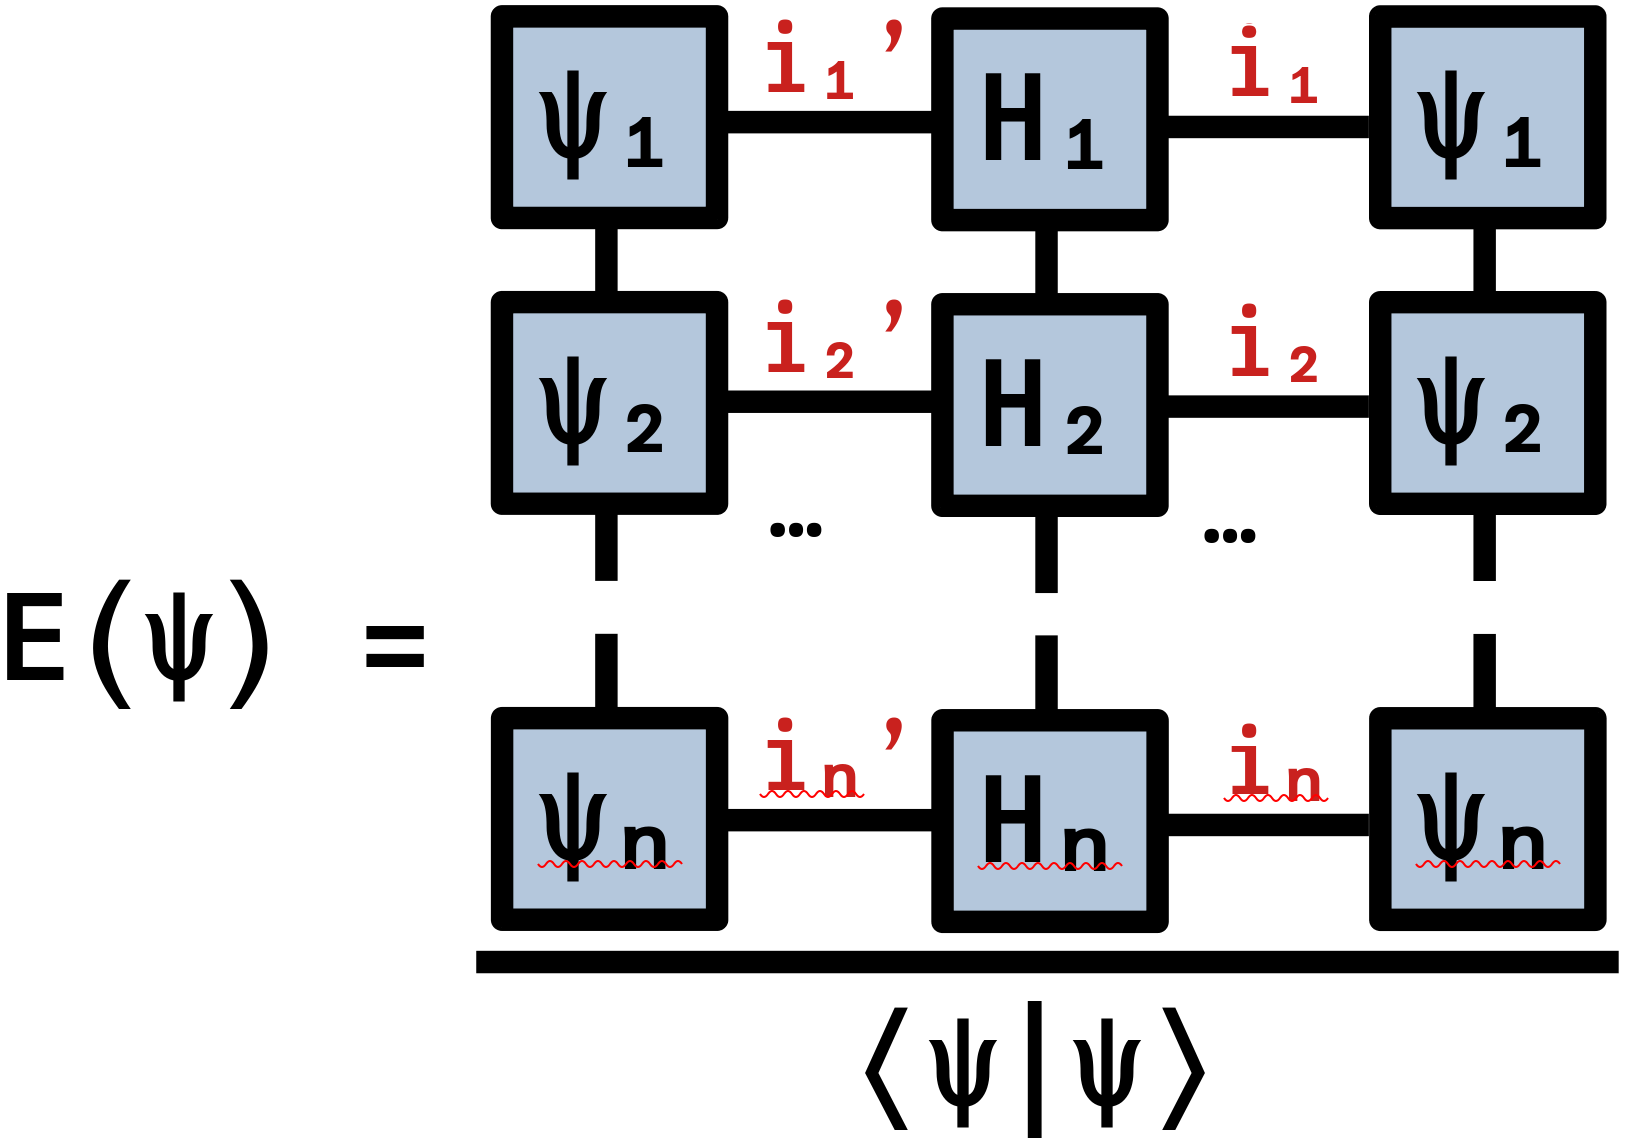
\includegraphics[width=0.8\textwidth]{
  slides/assets/psin_H_psin.png
} \\
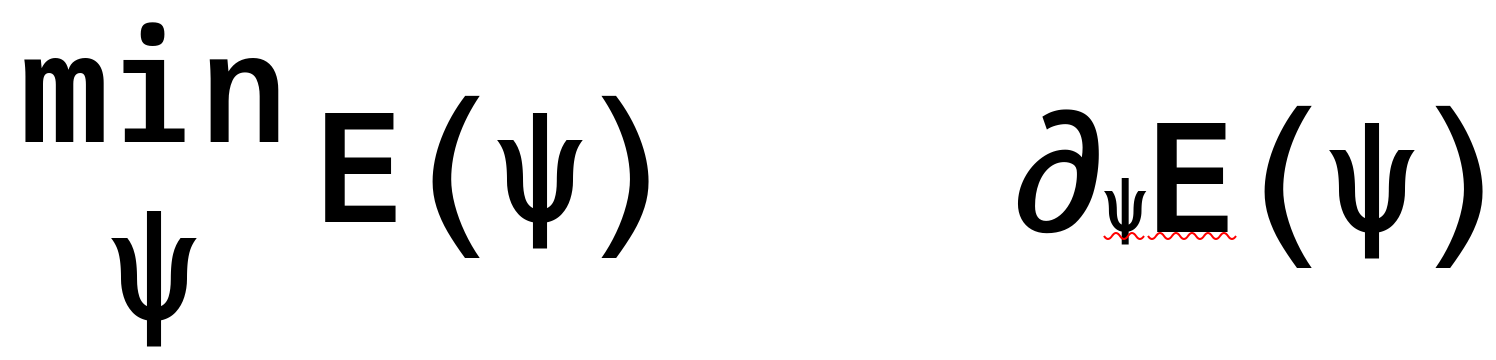
\includegraphics[width=0.7\textwidth]{
  slides/assets/min_grad_E_psi.png
}
\end{center}
\vspace*{0.0cm}
\end{onlyenv}

\begin{onlyenv}<3->
\begin{lstlisting}[language=JuliaLocal, style=julia, mathescape, basicstyle=\scriptsize\ttfamily]
maxlinkdim($\psi$0) == 1
maxlinkdim($\psi$) == 3
maxlinkdim($\psi_{dmrg}$) == 3
E($\psi$0) == -29
E($\psi$) == -31.0317917
E($\psi_{dmrg}$) == -31.0356110
\end{lstlisting}
~\\
~\\
\end{onlyenv}

%% \begin{onlyenv}<3->
%% = 1 (product state) \\
%% = 3 (entangled state) \\
%% = 2 (entangled state) \\
%% $\approx$ (-29, 5.4772256) \\
%% $\approx$ (-31.0317917, 0.06673780) \\
%% $\approx$ (-31.0356110, 0.02413237)
%% \end{onlyenv}

\end{column}

\end{columns}

\end{frame}
